% $Rev: 356 $:			Revision of last commit
% $Author: mg483 $:		Author of last commit
% $Date: 2018-05-24 16:05:25 +0100 (Thu, 24 May 2018) $:    Date of last commit

\documentclass[twoside,12pt,titlepage,a4paper]{article}
\usepackage{url}
% kentHarvard requires natbib
\usepackage{natbib}
% add line numbers
% TODO: remove line numbers and run minted for release
\usepackage{lineno}
% \usepackage{minted}
\usepackage{etoolbox}
\makeatletter
\patchcmd{\@verbatim}
{\verbatim@font}
{\verbatim@font\scriptsize}
{}{}
\makeatother
\usepackage[final]{pdfpages}
\usepackage{xcolor}
\linenumbers
\definecolor{periwinkle}{rgb}{0.8, 0.8, 1.0}
\renewcommand{\linenumberfont}{\normalfont\bfseries\small\color{periwinkle}}
\usepackage[pass]{geometry}
\usepackage{graphicx}
\renewcommand{\baselinestretch}{1.3}
\usepackage{todonotes}
% An empirical comparison of the structure of configuration files of continuous integration and build systems
\title{Usage and structure of continuous integration as configuration?}
\author{Joseph Ling\\\vspace{10mm}
\url{jl653@kent.ac.uk} \\ \vspace{5mm}

\includegraphics[scale=0.6]{Kent_Comp_294_RGB} \\
School of Computing \\
University of Kent \\
United Kingdom \\ \vspace{10mm} \\ Word Count: 6,100}
\begin{document}

\newgeometry{hmarginratio=1:1}    %% make layout symmetric
\maketitle
\restoregeometry              %% restore the layout

\begin{abstract}
  This paper describes a simple heuristic approach to solving large-scale
  constraint satisfaction and scheduling problems.  In this approach one
  starts with an inconsistent assignment for a set of variables and
  searches through the space of possible repairs. The search can be guided
  by a value-ordering heuristic, the {\em min-conflicts heuristic}, that
  attempts to minimize the number of constraint violations after each
  step.  The heuristic can be used with a variety of different search
  strategies.  We demonstrate empirically that on the $n$-queens problem, 
  a technique
  based on this approach performs orders of magnitude better than
  traditional backtracking techniques.  We also describe a
  scheduling application where the approach has been used successfully.  A
  theoretical analysis is presented both to explain why this method works
  well on certain types of problems and to predict when it is likely to
  be most effective.
\end{abstract}

\section{Introduction}
\label{Introduction}

https://arxiv.org/ftp/arxiv/papers/1703/1703.07019.pdf

Continous integeration (CI) is becoming more popular over the last few years. This can be seen by how major version control hosting services Github, Bitbucket and Gitlab have all started to or have been improving their CI product. In terms of research, configuration as code \cite{Rahman2019} and continuous integeration \cite{Copeland2010} with \cite{Shahin2017} demonstrating breadth of the research.

Continous integeration is a process of automatically running compiling, running tests and checking that the product works. This is can be combined with Continous Delivery where the product is deployed or released after it has gone through CI. 

This can get complicated quickly therefore configuration as code (or infrastructure as code) is used to configure it. The main kind of configuration format used for this is yaml (reference to what it is??) followed by xml and java based scripting formats.


In terms of looking at usage we are going do a similar look at the data as did \cite{Hilton2016}. The importanat aspect will be looking at how usage has changed over the last 5 years along with looking more closely at which repositories are more likely to use CI/CD. For this we are going to focus on the following research questions:
\begin{itemize}
  \item What percentange of open-source projects use CI?
  \item multiple CI used
  \item what is the breakdown of usage of different services?
  \item Do certain types of projects use CI more than others?
\end{itemize}

This should give us a better understanding of the sample of repositories from Github. From there we look at the structure of the configuration files to understand how certain aspects of it are used.
\begin{itemize}
  \item configuratizon errors when loading the config (just yaml parsing errors atm)
  \item how are comments used in the configuration?
  \item how scripts with the configuration files? (need to elloborate more on this one)
\end{itemize}

A key aspect is that these questions do not look too deeply into the individual implementation of each CI system. This is because there are already some good papers looking \cite{Gallaba2018} at this but in order to be able to compare the different configuration types it is important to compare similar attributes (there is also a time factor in here as well). 

\section{Previous Works}
\vspace*{-0.05in}
\subsection{Continous integeration}
\vspace*{-0.05in}

Continous integeration is the frequent submission of work normally tied into a feedback loop. For example using version control daily committing changes. That then a server builds and tests the changes informing you of status of those cahnges. The generally agree upon detailed definition is \cite{CI2010_MartinFowler}.

\vspace*{-0.05in}
\subsection{Usage of continous integeration}
\vspace*{-0.05in}

The actual usage of continous integeration as configuration was looked at by \cite{Hilton2016}. In this they use three source of information github repositories, travis builds and a survery. In order to be do a more systematic study of CI usage than \cite{Vasilescu2015}. In analysing that data they found that "The trends that we discovered point to an expected growth of CI. In the future, CI will have an even greater influence than it has today.". As we are looking at the same question we will use four of the same research questions out of the fourteen. In order to see what difference four years has made to the growth of usage of CI.

\vspace*{-0.05in}
\subsection{Config as code}
\vspace*{-0.05in}

Configuration as code or infrastructure as code has been an increasing area of research over the last few years. There seems to be slightly more research in infrastructure as code \cite{Rahman2019}. The has been a focus on Puppet and Chef, for example in \cite{Sharma2016} looks at code quality by the measure of "code smell" of Puppet code. This tackles the problem by defining by best practices and analyzing the code against that. In the case of \cite{Cito2017} it uses the docker linter in order to be able to analyse the files. 
For the continous integeration systems we pick we will look into the tooling around that to aid the analysis.


\section{Methodology}
\label{methodology}

In order to get repositories with CI/CD configuration from Github we have a number of approaches. The first is too use the search for particular files but this is limited to only 1000 results. The alternative is to search for repositories and we bypass the 1000 result limit to an extent by getting results for every 'star' count (stars are used to like or upvote a repository). Although this will be giving us a lot of results it will still only be a sample of the population but will give us a wider range of results. As their is rate limiting multiple github api keys can be used to speed up the scraping of data (ghtorrent could also be used to speed up the process I think).

After we have got a repository we need to get the CI/CD files from it. This is fairly easy as the CI/CD systems normally require a strict naming convention and location within the repository. However as most of them are yaml based you can have ".yml" and ".yaml" and users can use all sorts of mixtures of upper and lower case. We try to account for this but won't get every scenario. This combined with the fact that we are only looking for top configuration files based on \cite{Github2017} along with github actions and azure pipelines. Is why we also check repositories for their ReadMe.md file to check if it has a build tag.

\begin{figure}[h]
  \centering
  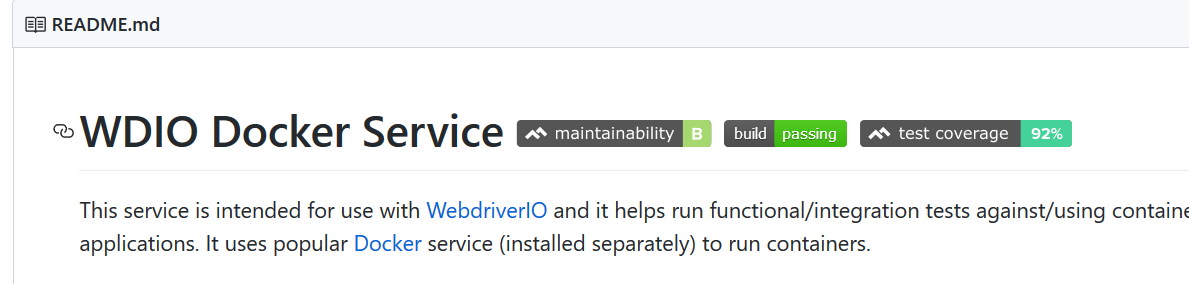
\includegraphics[scale=0.5]{2020-01-30-08-29-04.png}
  
  \caption[alt text]{Example of CI tag for Github ReadMe}
  \label{ExampleGitHubReadme}
\end{figure}

\todo[size=\scriptsize]{where did this image come from?? reference it man}

In doing so it should give a wider net when sampling and help to understand when a CI system is either not using configuration as code or using a different CI system.

There are dangers in scraping data off github in terms of assumptions to do with the population as found in \cite{Kalliamvakou2014}. Our dataset does not contain any forked repositories. But due to time constraints number of commits and frequency of recent commits has not been looked at. This would be an interesting area of further research in order to improve the quality of the sample but also to look at how that affects the frequency of CI usage.

Additionally the assumption that all repositories are of programming projects with code in them is wrong. A number of repositories can be used for storage, experimental, academic and other things. However they to all some extent can use CI/CD for their work as a number of books were found when looking through the dataset could use CI/CD.

Tooling for the configuration files, I looked into Travis, Github Actions and Jenkins to work out whether or not it could aid in the research or not. As a key part of understanding the first relies on knowing whether or not it is valid. 
In terms for travis there is currently two parsers to validate the configuration. One which is depracted since 2017 \cite{TravisYamlParserOld2017} the other which is currently in development \cite{TravisYamlParserNew2020}. Both didn't provided the necessary results with the most recent one not being able to handle default fields.
For Github Actions as it's still a new tooling for it hasn't been developed outside of the Github editor web page (https://github.community/t5/GitHub-Actions/YAML-validator-for-Github-Actions-possible-expansion-of/td-p/29557).
For Jenkins which is older solution allows validation through http/ssh request to the Jenkins server (Gitlab follows this style as well) \cite{JenkkinsDocs2020} \cite{GitlabDocs2020}. This could work well although would require setting up a server for each configuration type and might not validate if varaibles from the config aren't defined on the server. As well as it would be best to be able to validate them all or none of them in terms of being able to compare results easily.

\section{Usage of CI}

\vspace*{-0.05in}
\subsection{What percentange of open-source projects use CI?}
\vspace*{-0.05in}

Based a search for configuration as configuration files for the following CI systems: Travis, Gitlab, Azure, App Veyor, Drone, Jenkins, Github, Circleci, Semaphore, Teamcity and buildkite. 
Wrecker got bought by Oracle and from doing a search on Github for what I think based on the docs (docs: \cite{WreckerDocs} and search: \cite{WreckerOpenSourceGithubSearch}) for their config file naming convention. I was only able to find 20 results so did not include in the scraping script to speed up the process of searching for the other configuration file formats.


    \begin{table}[h]
\begin{tabular}{|l|l|l|l|l|}
\hline
    CI/CD & \textbf{count} & \textbf{repos with config} & \textbf{no. multiple} & \textbf{multiple percent}   \\ \hline
config file(s) &           12128     & 38.51\%                                & 1675          & 13.81\%             \\ \hline
found in ReadMe & 873     & 2.77\%                                &             &             \\ \hline
none found &            18493     & 58.72\%                                &             &             \\ \hline
\end{tabular}
\caption[Percentage of CI used for projects]{Percentage of CI used for projects}
\end{table}
    

Our sample of repositories is 31,494 in comparison to \cite{Hilton2016} which had a sample of 34,544. The percentage of CI projects they had was 40.27\%. As if you combined the "config file(s)" and "found in ReadMe". However in order to work out if a project might be using CI but the config file wasn't picked a search string is used. Therefore it is not as accurate as finding a config file as their could be false postives.

However that doesn't give us too much insight into the dataset. Here is a graph showing the subscribers plotted against the number of stars. The key here to understand is not potentially any correlation but to see the spread of data that the table is showing. 

\begin{figure}[h]
  \centering
  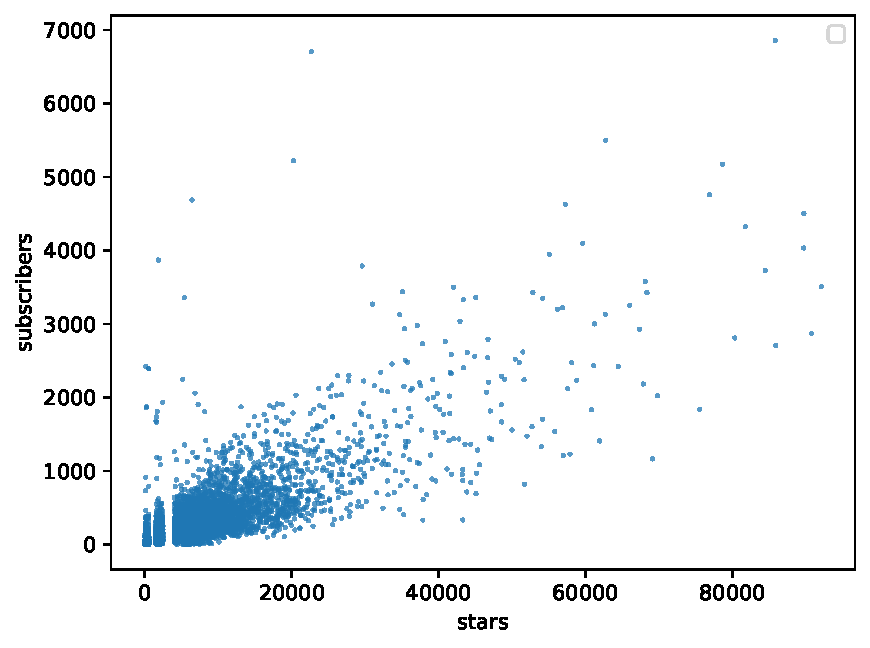
\includegraphics[width=\textwidth]{../src/results/sub vs stars.pdf}
  \caption[alt text]{Scatter graph of Github stars against subscribers}
  \label{graph_scatter_stars_vs_subs}
\end{figure}

Figure \ref{graph_scatter_stars_vs_subs} helps give a understanding to the give a depth of the data for where the graph is just blue. This is because on Github you get more repositories with smaller star counts than large ones.

\begin{figure}[!htbp]
  \centering
  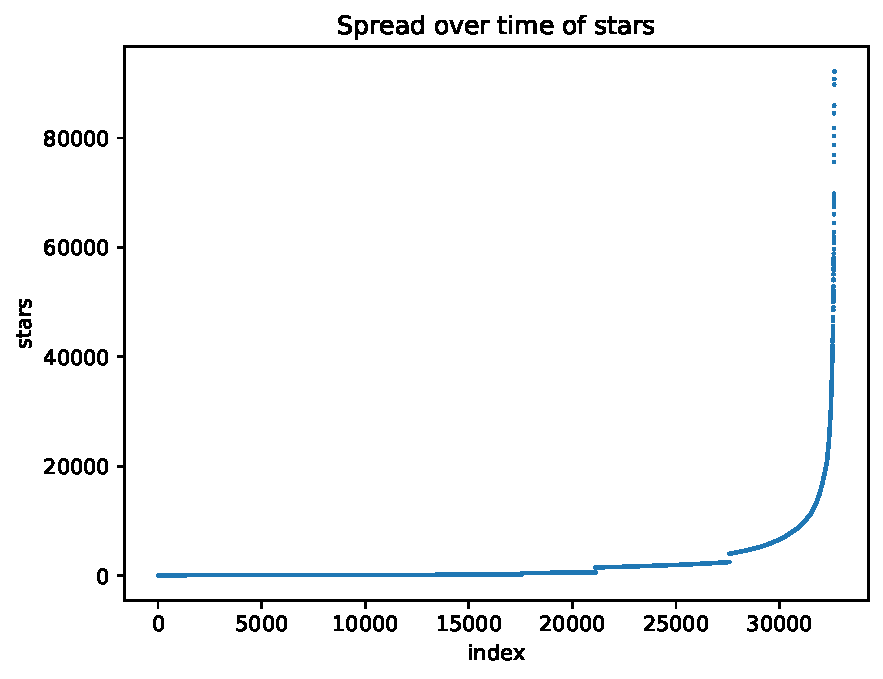
\includegraphics[width=\textwidth]{../src/results/spread over time.pdf}
  \caption[alt text]{Stars graph}
  \label{graph_scatter_stars_line}
\end{figure}

Figure \ref{graph_scatter_stars_line} provides insight into the density of the data for between 0 to 25000.

\vspace*{-0.05in}
\subsection{What CI systems are projects using?}
\vspace*{-0.05in}
Like all other research travis is the most popular CI system in use. However over the last 4 years since the \cite{Github2017} Circleci has lost out on it's rough quarter that it owned. In particular the rise of github actions seems to have taken second place even though it is still very young in comparison (DATES). However this might not be down to the Circleci loosing out on their existing share. But potentially as the rise in CI usage goes up on github. Projects are more likely to pick in the built in solutions to github.
\begin {table}[!htbp]

\caption{Configuration types spread}
\label{table_config_types}
\begin{tabular}{lrl}
\hline
{} &  config & percentage \\ \hline

Travis          &   10607 &        74\% \\ \hline
Github          &    2301 &        16\% \\ \hline
CircleCi        &    1109 &         8\% \\ \hline
Jenkins pipeline &     161 &         1\% \\ \hline
Drone           &      84 &         1\% \\ \hline
Buildkite       &      32 &         0\% \\ \hline
Teamcity        &       4 &         0\% \\ \hline
Semaphore       &       2 &         0\% \\ \hline
Azure pipeline           &       1 &         0\% \\ \hline

\end{tabular}
\end{table}


\pagebreak
\vspace*{-0.05in}
\subsection{Do certain types of projects use CI more than others?}  
\vspace*{-0.05in}

Below shows all the CI projects sorted then grouped together per 540 projects. Then in this case we choose to categories via star count for each project. 

\begin{figure}[!htbp]
  \centering
  \begin{minipage}{.48\textwidth}
    \centering
    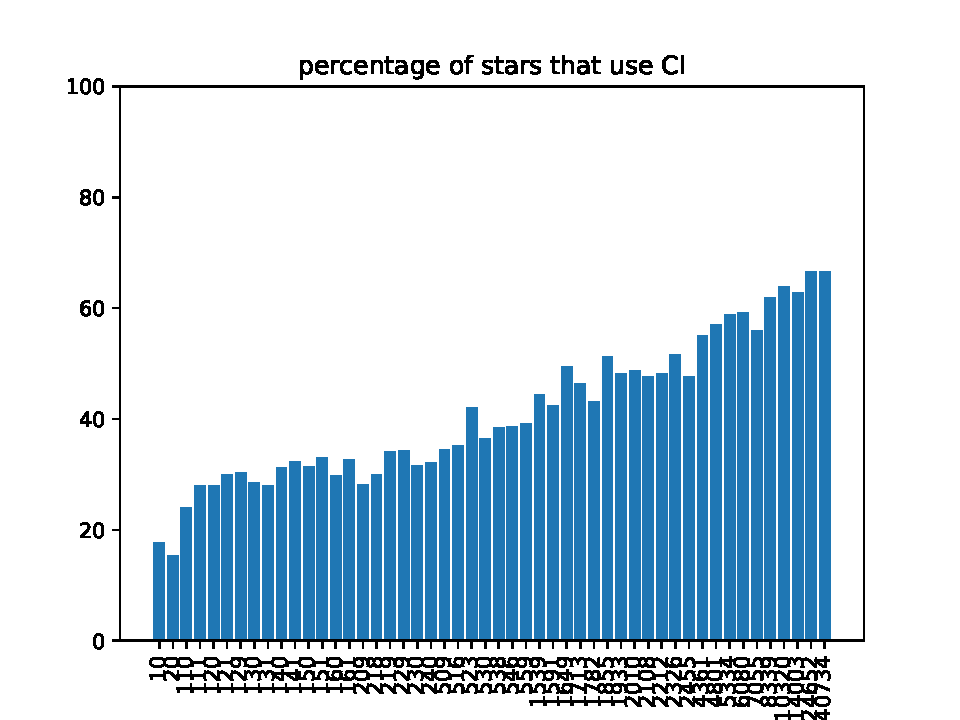
\includegraphics[width=.9\textwidth]{../src/results/percentage stars with CI.pdf}
    \caption{2020 dataset}
    \label{fig:test1}
  \end{minipage}%
  \hfill
  \begin{minipage}{.48\textwidth}
    \centering
    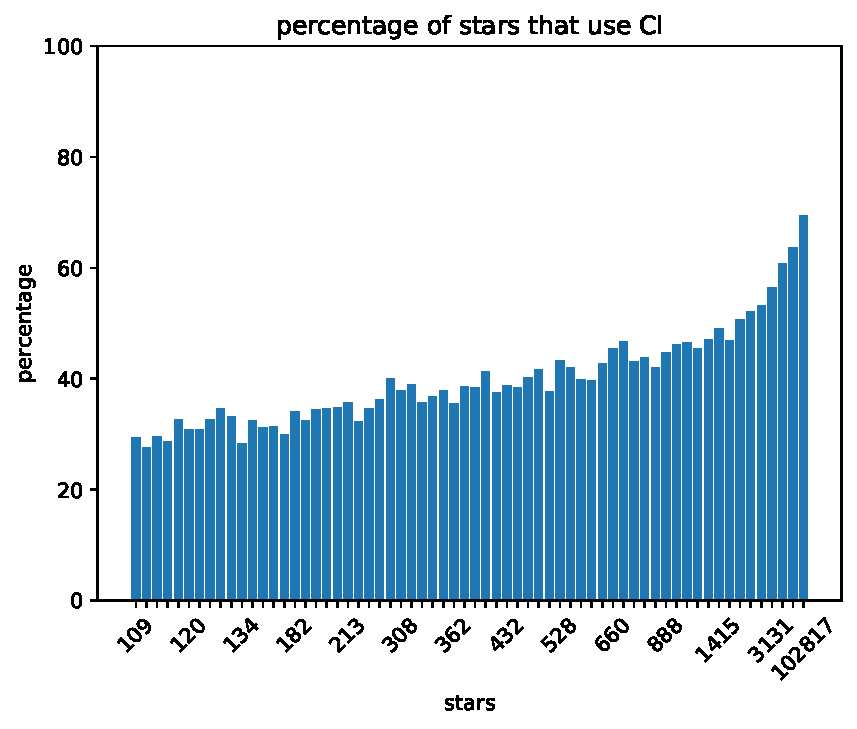
\includegraphics[width=.9\textwidth]{../src/results/percentage sub with CI other paper source.pdf}
    \caption[]{2016 dataset}
    \label{fig:test2}
  \end{minipage}
  \caption{In Figure \ref{fig:test1} is the results from this research and in Figure \ref{fig:test2} is the results from \cite{Hilton2016}.
  }
\end{figure}

Here we are comparing whether or not in the last 4 years the number of stars increases the CI being used. Their seems to a steeper gradient in the more recent datasets. However as \ref{fig:test1} starts at zero stars and \ref{fig:test2} starts at 100 stars their is signifacant dip at the start of the first graph.

\begin{figure}[!h]
  \centering
  % TODO: make this bigger when the time comes
  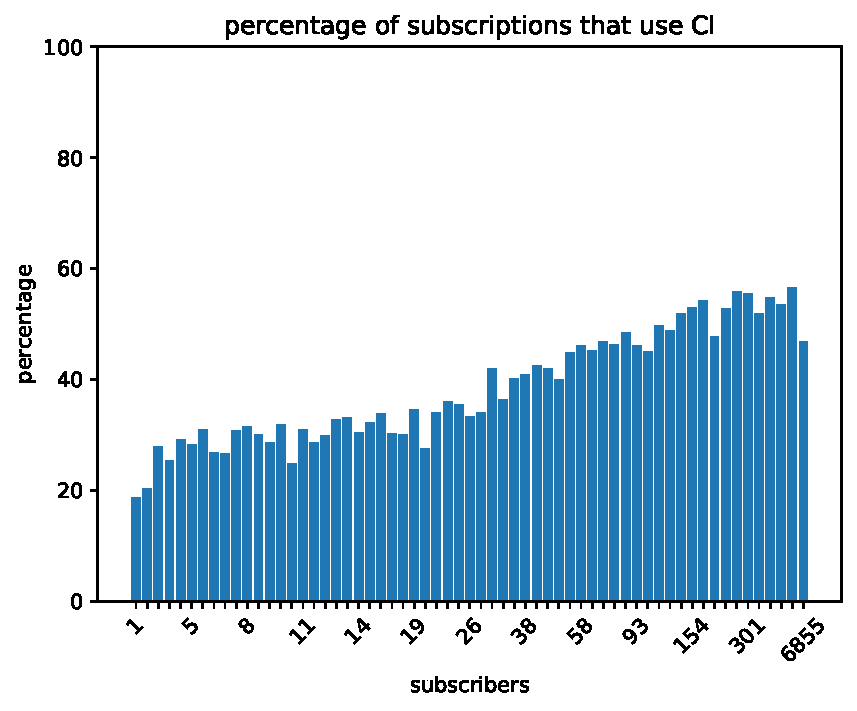
\includegraphics[width=.3\textwidth]{../src/results/percentage sub with CI.pdf}
  \caption{Subs graph}
  \label{graph_percentage_subs}
\end{figure}

Figure \ref{graph_percentage_subs} uses the same method as Figure TODO SORT except is does it based the number of subscribers. Subscribers are used on github to keep update on the changes on the project. This ranges from core team memembers working on the project to people that want to be notified about a new release. 
In looking at this metric the hypothesis was that it would have a sharper rise in percentage of projects using CI per subscriber. However that was not the case overall the gradient is not as strong. There is no comparisson to \cite{Hilton2016} because their final corpus does not contain subscriber count for each project.






\section{Config file results}

\vspace*{-0.05in}
\subsection{configuration errors when loading the config (just yaml parsing errors atm)}
\vspace*{-0.05in}

\begin{figure}[!h]
  \centering
  \begin{minipage}[t]{.48\textwidth}
    \textbf{Composer error}
    In the example it has two steps that are using an yaml anchor. This allows for the yaml below it to be referenced somewhere else. However if you define the anchor twice it causes a composer error. As you have two references for the samething so it won't know which one to use.
  \end{minipage}%
  \hfill
  \begin{minipage}[t]{.48\textwidth}
    \begin{verbatim}
      definitions: 
      steps:
      - step: &build-test
      name: Build and test
      script:
      - mvn package
      - step: &build-test
      name: deploy
      script:
      - ./deploy.sh target/my-app.jar
    \end{verbatim}
  \end{minipage}
\end{figure}

\begin{figure}[!h]
  \centering
  \begin{minipage}[t]{.48\textwidth}
    \textbf{Scanner error}
    The first step of loading the yaml is to scan it to create the tokens. However invalid characters such as "\textbackslash t" are invalid. 
  \end{minipage}%
  \hfill
  \begin{minipage}[t]{.48\textwidth}
    \begin{verbatim}
      definitions: \t
    \end{verbatim}
  \end{minipage}
\end{figure}
\begin{figure}[!ht]
  \centering
  \begin{minipage}[t]{.48\textwidth}
    \textbf{Parse error}
    In this example it has scanned the file and created tokens for the syntax. Now it parses the syntax and works out if each token is valid given it's current context. In this case a closing ] without an opening [ is invalid.
  \end{minipage}%
  \hfill
  \begin{minipage}[t]{.48\textwidth}
    \begin{verbatim}
      definitions: ]
    \end{verbatim}
  \end{minipage}
\end{figure}

\begin {table}[!htbp]

\caption{cats}
\begin{tabular}{|l|l|l|l|}
\hline
\textbf{yaml\_encoding\_error} &  composer error &  parse error &  scanner error \\ \hline
\textbf{config  } &                 &              &                \\ \hline

\textbf{circleci} &               0 &            0 &              1 \\ \hline
\textbf{drone   } &              30 &            0 &              0 \\ \hline
\textbf{github  } &               0 &            0 &              3 \\ \hline
\textbf{travis  } &               6 &           10 &             21 \\ \hline

\end{tabular}
\end{table}


As can be seen in the table their our configuration files with yaml errors meaning that the CI for that project will not load. Yet it seems that a very small percentage of projects that have them. For example the two highest configuration types with errors are drone (36.90\%) followed by travis (0.348\%).

In the case for drone all the errors are for the same type of error. Potentailly this could be because of how anchors are a lot more common in drone.

For travis it is the most common form of CI found therefore it is more likely to contain more errors. Yet with such a small amount it seems like yaml errors aren't a major problem in CI. Although as they are required to be fixed in order for the CI to run the chances of it working are higher and a more detailed study would need to be done.... ah


\pagebreak

\begin{figure}[!ht]
  \vspace*{-0.05in}
  \subsection{How are comments used in configuration?}
  \vspace*{-0.05in}
\end{figure}


The assumption was the as continuous integeration setups can be complicated and have edge cases. Therefore comments would be used to describe and handle that complexity.

An example configuration file below for Github actions using the default template slightly altered. Shows two examples of comment usage, the first being including useful information about why a particular version of the programming language was chosen. The second is that the tests have been disabled by commenting them out. 



\begin{figure}[!htbp]
  \centering
  \begin{minipage}[t]{.48\textwidth}
    In order to pick up on all these different types of comments. All the CI files were parsed and then regular expressions were used to pick on up key factors such as "note:". Along with multiple single line comments which made up a block/multi-line comment.
    
    For example in to the left there is an example Github Action yaml file. If were it would be parsed we would get: one multi line comment, 15 lines of code, 1 single line comment, a total of 5 comments and 20 lines in the file. Therefore their is a their is a raito of 4:1 for code in this config file.
  \end{minipage}%
  \hfill
  \begin{minipage}[t]{.48\textwidth}
    \begin{verbatim}
      name: Python package
      on: [push]
      jobs:
      build:
      runs-on: ubuntu-latest
      steps:
      - uses: actions/checkout@v2
      - name: Set up Python
      uses: actions/setup-python@v1
      # note: only works with python 3
      with:
      python-version: 3.8
      - name: Install dependencies
      run: |
      python -m pip install --upgrade pip
      pip install -r requirements.txt
      #      - name: Test with pytest
      #        run: |
      #          pip install pytest
      #          pytest ./src
    \end{verbatim}
  \end{minipage}
\end{figure}

% NOTE: NEED TO EXPLAIN CODE_WITH_COMMENTS

Initally before we look at the comments it is important to understand how the rest of the file is made up. In the graph below (Figure \ref{fig:bar_comments_lines}) it shows how each configuration type is made up by mean of each part of the file. For all the yaml based configurations lines of code and number of lines in total are very close. Then for the number of commments being very very small on average.

In the case for Jenkins pipelines and teamcity there is a much higher usage of having code with commments. 


\begin{figure}[!ht]
  \centering
  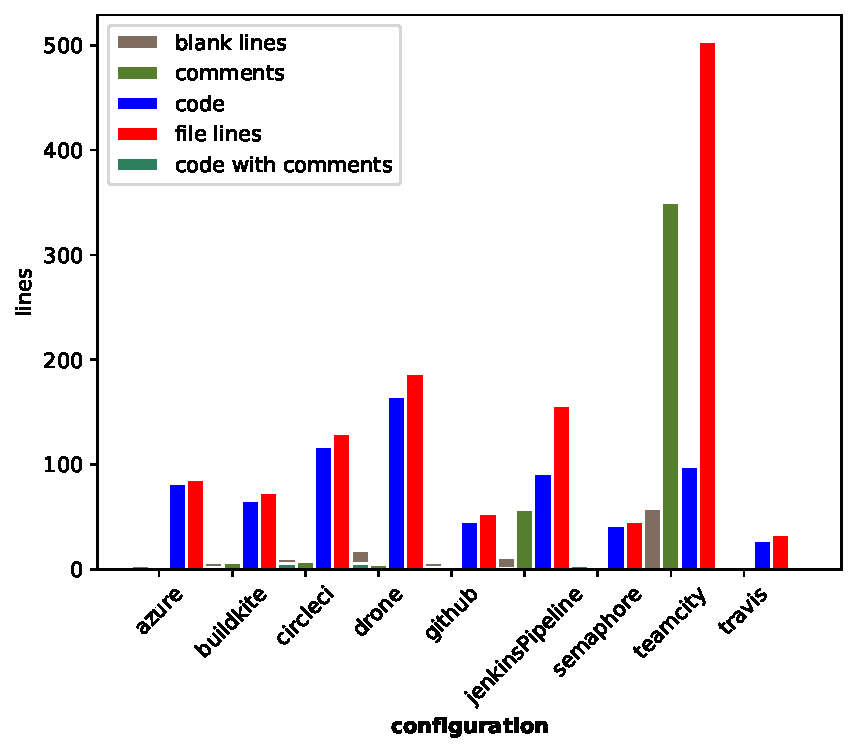
\includegraphics[width=\textwidth]{../src/results/basic comments bars.pdf}
  \caption[alt text]{Mean of line counts}
  \label{fig:bar_comments_lines}
\end{figure}

Raitos:
\begin{itemize}
  \item{code: comments}
  \item{code: line total}
  \item{code: blank lines}
  \item{single line comment: multiline comment}
  \item{single line comment: code with comment}
\end{itemize}






\begin{figure}[!ht]
  \centering
  \begin{minipage}[!t]{.48\textwidth}
    In Figure \ref{fig:comment_types} a regular expression was used to label the comments. There were key different types of comment that we wanted to find. The first being the commented out code which we did by searching for version numbers in commments. The second being useful information about the structure of the CI file such todo, note, importanat comments (e.g. //todo). In order to increase the search for this we included searching for urls and seperation comments (e.g. //===).
    
  \end{minipage}%
  \hfill
  \begin{minipage}[!t]{.48\textwidth}
    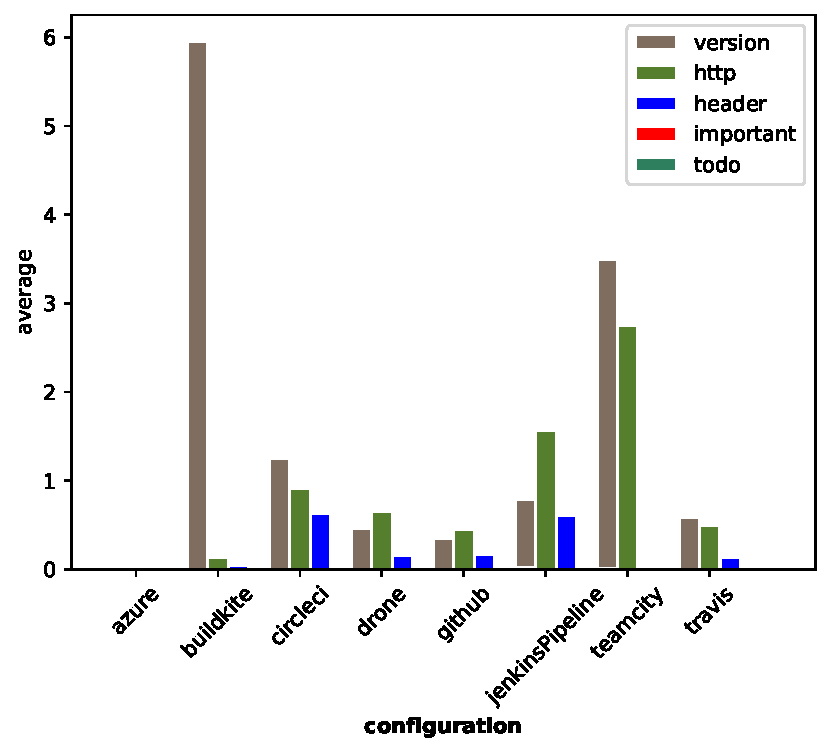
\includegraphics[width=\textwidth]{../src/results/comments usage bars.pdf}
    \caption[alt text]{Comment types}
    \label{fig:comment_types}  
  \end{minipage}
\end{figure}

From labelling the comments in Figure \ref{fig:comment_types} we can see that having commments with versions in and urls is most common. This could indicate comments from templates or how they are commented. Although yet again the amount of labels found on average is still very low.

Overall we have found that comments are not used a lot. In the cases that they are used it's more likely to be from a configuration template or commenting out configuration.
% NOTE: update this when raitos are done

\pagebreak

\vspace*{-0.05in}
\subsection{How are script tags used?}
\vspace*{-0.05in}

- how scripts with the configuration files? (need to elloborate more on this one)

\section{Threats to validatity}

strength and validaltiy section 
- possible issues
- baise assume in the data
- e.g. sampling vai star
- focusing on github
- problematic of scraping tool





\section{Summary}

asdfasdf

55df26ae2061a09c5830423efc280783897fe8c9
\vspace*{-0.05in}
\subsection{Discussion and further research}
\vspace*{-0.05in}
In the process of writing this paper we kept on considering more research questions. As there is a lot of meta data that you can get for a single project, in addition to what was used for this paper.

Further research into usage that we would like to do is look into how the size of the project affects the chance that it uses CI. Then looking at the usage of scripts within CI configuration, for example using a script tag to run a shell script. As while doing the research we found some projects use scripts a lot while others just used the CI config. This would lead to questions around which CI system has a higher amount of scripts used. But also looking at how much they enable them to be used and what is the size of those scripts.
The data for the programming language and version(s) is in the config. Therefore it would be possible to work out how much usage each version is getting of a particular programming language.

Further research into structure could look into the naming of each part of the build process that is used. This would be interesting as it would provided insight into what terms are commonly used. As well an idea into how people plan or don't plan out their configuration files.
Additionally CI systems can be designed to run on every commit to version control or only commits to certain branches. Therefore by looking at the branching regexp that are being used an better understanding of how branches are actually used in software development where CI is also used could be found out.

In addition working on pruning our dataset using methods outlined in \cite{Kalliamvakou2014}. 


% After looking at these results three areas of research that could be interesting would be filtering the sample to only projects that had recent commits. On the assumption that CI is becoming more popular and stale projects won't require CI.

% Looking into whether or not that assumption is the case. Then looking commit count to see if projects with more commits are more likely to use CI.

\section{Acknowledgement}
The authors wish to thank Hans-Martin Adorf, Don Rosenthal, 
Richard Franier, Peter Cheeseman and Monte Zweben for their assistance
and advice.  We also thank Ron Musick and our anonymous reviewers for
their comments.  The Space Telescope Science Institute is operated by
the Association of Universities for Research in Astronomy for NASA.

\appendix
\section*{Appendix A. Probability Distributions for N-Queens}


[section ommitted]



\vskip 0.2in
\bibliography{sample}
\bibliographystyle{kentHarvard}

\end{document}
